\documentclass{wrcecapstone}
% wrcecapstone.cls file can be obtained using
% git clone ssh://git@github.com/devangel77b/wrcecapstone.git 
% and putting the file in your texmf tree

\usepackage{graphicx} % for graphics
\usepackage{svg}
\usepackage{siunitx} % for units
\usepackage{listings} % for code
\lstset{basicstyle=\small\ttfamily}
\usepackage{booktabs} % for pretty tables

% if using IEEE type references
\usepackage{cite}
% if using biology style references
%\usepackage[round,authoryear]{natbib}

\newcommand{\Matlab}{Matlab} % in case your advisor prefers Matlab versus MATLAB

\title{Template for EW402/4 Capstone Report}

\author{Midshipman 1/C Alyssa P. Hacker and Midshipman 1/C Benjamin Bitdiddle}
%\contactinfo{aphacker at alum dot mit dot edu}
%Optional contact information: consider including civilian e-mail addresses in case a group from next year’s class would like to continue your project and would like to contact you with questions.

%\advisor{Assistant Professor Indiana Jones}
\departmentchair{Professor Brad Bishop}
%\outsidesponsor{Professor Bigshot Arr One}
\date{May 5, 2018} % fill in the date you intend to hand it in!




\begin{document}
\maketitlepage
\cleardoublepage
\tableofcontents
%\listoffigures
%\listoftables

%first page
\clearpage
\maketitle
\begin{abstract}
Your abstract should summarize the objective of your capstone project, briefly explain its importance in context of the broader engineering landscape, summarize the final design and highlight significant results or performance measures.
\end{abstract}

\section*{Preface: Using the template}
\LaTeX\ is a document preparation language widely used in scientific and engineering academic publication.  You will need to install \LaTeX\ on your system; we suggest the Miktex distribution \url{https://miktex.org/} on Windows machines. The class files can be obtained from \url{https://github.com/devangel77b/wrcecapstone}; they are installed in your \lstinline{texmf} tree. 

Use \LaTeX\ sectioning commands in order to automatically get the correct heading styles for \lstinline{section}, \lstinline{subsection}, and \lstinline{subsubsection}. The * versions of these commands are not numbered and are omitted from the table of contents by default. Use \lstinline{figure} and \lstinline{table} environments to define figures and tables, respectively. Use \lstinline{cite} to provide citations to references. You can also use the \lstinline{footnote} command.  

See Appendix~\ref{app-style} for tips on inserting figures, captions, tables, and equations, as well as some general technical writing tips and style guide information.  Delete this preface section from your final report. Using \LaTeX\ will save your advisor time later if your work is to be reformatted and published as a conference or journal article; it also frees you from worrying too much about the formatting as \LaTeX\ handles such things automagically. 

The sections in this template apply for an engineering design project. If your project is more closely patterned as a science project in which you are testing hypotheses, you and your advisor may choose to organize the report differently. 
%PREFACE: Using the Template
%Duplicate this template file by using the Save As command.  Save the new file as a Word document (.docx) rather than a template (.dotx).  Choose a filename that begins with “ES404_” followed by a short project title and your class year. 
%This electronic document1 is a “live” template. The various components of your paper (title, text, heads, etc.) are already defined on the Style Toolbar above and are illustrated throughout the template.  Please do not change font type, size or page layout.   
%The Heading Styles help organize the topics on a relational, hierarchical basis. For example, the Title Style is the primary heading because all subsequent material relates and elaborates on this one topic. If there are two or more sub-topics, the next level heading should be used (i.e. Styles named “Heading 1”, “Heading 2”, “Heading 3”, and “Heading 4” in the Style Toolbar). Conversely, if there are not at least two sub-topics, then no subheads should be introduced. 
%Using the styles will facilitate the automatic creation of the Table of Contents.  You can force the table to update using right-click Update Field Codes / Update Entire Table. 
%See the Appendix for tips on inserting figures, captions, tables, and equations in MSWord, as well as some general technical writing tips. 
%Delete this preface section from your final report. 




\section{Introduction}
In this section you have three main objectives to get across to a reader:  

\subsection{Motivation}
First, provide the reader with \textbf{background} information that motivates your overarching problem and discusses areas of potential impact.  Here you might cite societal, economic, political, or military events and trends.

\subsection{Problem Statement}
Second, present your \textbf{problem statement}.   Be succinct yet as specific as possible.  A photo or conceptual diagram is often useful (see Appendix~\ref{app-style} for tips on inserting figures and captions).   Avoid presenting the solution; that belongs in the next section.  Make it clear how your problem statement addresses a need of the overarching problem and the possible impact of a successful design.  If you have specific requirements from a customer or another stakeholder, be sure to include these in this section.

\subsection{Related Work}
Third, critically discuss and reference \textbf{similar products or research by others}.  Critique their solutions, explicitly stating what attribute you tried to emulate or shortcomings you tried to improve upon.  Be sure to read the guidance on inserting citations and references.





\section{Design Process}
In this section your main goal is to explain your design process. Use figures to support the discussion and explanation of your design process.
 
\subsection{Customer Interviews and Requirements Generation}
Discuss how you conducted your customer interview(s) and the primary feedback and insight you gained during the interview process.  Review the list of customer requirements and how you prioritized them.  Discuss any competing requirements and how you plan to handle these.

\subsection{Functions and Morphological Chart}
Discuss the functions that were developed during Conceptual Design and provide a description or drawing for each.  Include your Morph Chart(s) and discuss the various options for each function and subsystem as well as how you made your component selections.

\subsection{Decision Matrix and Preliminary Design}
Include your final decision matrix and a detailed summary of your preliminary design.  Pictures are good here.  Make sure to include callouts and clarifying information for the graphic.

\subsection{Ethical Considerations}
Briefly discuss ethical issues that impacted your design approach.  Incorporate the \emph{IEEE Code of Ethics}\footnote{IEEE Code of Ethics is available online at \url{https://www.ieee.org/about/corporate/governance/p7-8.html}} or the \emph{Professional Engineer’s Code}\footnote{The NSPE Code of Ethics is availble online at \url{https://www.nspe.org/resources/ethics/code-ethics}} into your discussion when possible. 

\subsection{Engineering Analysis and Prototype Development}
List and discuss any engineering assumptions used in your analysis. This section should also include your prototype development or mathematical models used to predict behavior and system performance.  If you used a simulation or other computer-aided design tools, discuss them here. 
%You could also discuss the accuracy of your analysis in the context of your assumptions. This section could include the development of a mathematical model and/or the use of a model to predict behavior and system performance.  If you used simulation or other computer-aided design tools discuss them here.

\subsection{Component Selection}
Explain how you selected components of your design, such as actuators, power supplies, computing resources, and sensors—update EW401 material, such as your morph chart, as needed.  

\subsection{Design Evolution}
Your final design may not be what you originally planned. If so, discuss this evolution.
 





\section{Final Design}

\subsection{Overview}
Begin with your functional block diagram and a picture of your completed design.   At the very least, present the mechanical, electrical and software sub-systems as shown below.  Consider making additional subsections to present other subsystems.   

\subsection{Mechanical Subsystem}
This section should discuss the materials used and the dimensions and assembly of all mechanical components. Photos should be annotated, captioned, and referred to within the text (see Figure~\ref{f1}). Simple dimensioned drawings may be included here, but could also be included in the appendix. Hand-drawn engineering sketches are only appropriate for the appendix, or in the case of scientific illustrations. Consider use of line art for clarity and especially when compared to low-quality cell phone images with cluttered backgrounds. When using photos, take care to remove distractions in the photo and provide correct lighting so that the photo is clear. 
\begin{figure}
\begin{center}
\includesvg[width=\columnwidth]{figures/f1.svg}
\end{center}
\caption{This is an example of a dimensioned mechanical drawing (left) and an annotated photo (right).  The figures are composed in Inkscape, saved as an \lstinline{.svg}, and included using the \lstinline{includesvg} command. Figures are created using the \lstinline{figure} environment in \LaTeX. The caption is added using the \lstinline{caption} command. \LaTeX\ automatically numbers the figures. Adding a \lstinline{label} allows you to automatically cross reference your figures.}
\label{f1}
\end{figure}

\subsection{Electrical Subsystem}
All necessary circuitry, signal conditioning components, power supplies and connections should be detailed.  Circuit diagrams should include component values (e.g. resistance) as shown in Figure~\ref{f2}. Photos should be annotated, captioned, and referenced within the text. Consider placing complex circuit diagrams in the appendix. Hand-drawn circuit diagrams are only appropriate for the appendix; schematics can be drawn in CAD programs like ExpressPCB and Eagle, or can be coded for \LaTeX\ using the \lstinline{circuitikz} package.   Include any calibration equations for your sensors or actuators in this section. 
\begin{figure}
\begin{center}
\includesvg[width=\columnwidth]{figures/f2.svg}
\end{center}
\caption{This is an example of an electrical circuit diagram (left), note the component values are included; and an annotated picture of a fabricated circuit (right).}
\label{f2}
\end{figure}

\subsection{Software Subsystem}
Within the text, your algorithm or controller design should be in the format of pseudo-code (see Figure~\ref{f3}). It is not necessary to include computer programs in their entirety, though interesting excerpts may be included in the text. Appropriately comment any included code. The documentation needs to clearly indicate what code was written by the group members versus code provided by another source (e.g. faculty, TSD, commercial or open-source software, etc.).  For larger, hierarchical programs, represent the functional organization with a flow chart or a block diagram.  For programs utilizing GUIs, screen captures of the user interface are useful.   
\begin{figure}
\begin{lstlisting}
MyProject = NotWorking; 

while (MyProject != Working)

  WorkHarder;
  WorkSmarter;

end
\end{lstlisting}
\caption{Pseudocode is one of the most compact ways to present computer programs. Pseudocode and formatted code with syntax highlighting can be included in \LaTeX\ using the \lstinline{listings} package, using the commands \lstinline{lstinline}, \lstinline{lstlisting}, and \lstinline{lstinputlisting} for entire source files.}
\label{f3}
\end{figure}
  https://miktex.org/
\subsection{Feedback Control}
Present your control law as an equation or pseudo-code.   See the equation formatting guide in the appendix.  
\begin{equation}
\mbox{Throttle} = K (V_{des} - V)
\end{equation}

Justify how you selected its type (e.g.  open loop, bang-bang, proportional, state variable feedback, etc.). Provide values for the gains or coefficients.  Discuss their calculation and any iterative design procedure.  Provide plots, from either simulations or experiments, illustrating its effectiveness.  You can easily create feedback diagrams in Inkscape or Adobe Illustrator.  Resist the impulse to use Word or Powerpoint; the results look like crap. Once drawn, include your figures as shown in Figure~\ref{f4}.   You can include \Matlab\ figures as shown in Figure~\ref{f5}.
\begin{figure}[p]
\begin{center}
\includesvg[width=0.5\columnwidth]{figures/f4.svg}
\end{center}
\caption{Feedback control diagram. Please do not draw your diagrams using Word or Powerpoint artwork; figures done this way look like crap. Instead use a proper a drawing program like Illustrator or Inkscape; Inkscape is free. Use of scaleable vector graphic (\lstinline{svg}) format allows \LaTeX\ to typeset text within the figure.} 
\label{f4}
\end{figure}
\begin{figure}[p]
\begin{center}
\includesvg[width=0.75\columnwidth]{figures/f5.svg}
\end{center}
\caption{This is the response of the feedback control law.   Note that it is scaled appropriately to see the interesting features, and annotated.   When importaing \Matlab\ figures, you may need to set the export image size and increase the font size and line width to improve legibility. To make this repeatable, we recommend you include code to make the figure publication-quality when you first generate it; that way you can remake the figure with a minimum of fuss when you inevitably need to make small changes later.}
\label{f5}
\end{figure}





\section{Results and Analysis}

\subsection{Demonstration Plan}
This section documents a \textbf{procedure} for verifying the performance of your design including a list of required equipment, a list of all initial settings, controlled conditions and the commanded inputs to your system. If you used a test ``course'' or other apparatus, include a picture.  Someone should be able to replicate your experiments based on the instructions you provide in this section.  

\subsection{Performance Measures}
Evaluate your design against the performance measure rubrics, (i.e. your metrics) you developed in EW401. Discuss the extent to which you achieved each objective, striving to include \textbf{quantitative analysis} of your system’s performance. Examples include error, speed, settling time, time to set up, usability, etc. Where applicable use appropriate statistical procedures to analyze the data (this should include repeated trials). Use tables or graphs as appropriate to display more detailed results.  

Verify that your system satisfies the constraints outlined in the System Design section.




\section{Project Management}

\subsection{Work Breakdown Structure}
For capstone work involving more than one student, describe the distribution of the workload over the semester. Discuss any specialization or leadership roles in different disciplines, skills, or subsystems. Note that all group members contribute to the writing of the final report and presentation – it should not be one person’s job alone.  

\subsection{Life-long Learning}
As appropriate, briefly discuss any new knowledge that the team members acquired or developed over the course of the capstone project. This may include learning new hardware, software, or techniques.

\subsection{Cost analysis and Parts List}
Include it in tabular form (see the Appendix for tips on inserting tables).  Provide subtotals for parts alone, but also include labor\footnote{The usual way to account for labor in EW401 is by adding a fixed person-day cost for midshipman work. Your advisor may direct you to instead simply tabulate the person-day or person-hour effort so as not to provide artifically and unrealistically inflated cost estimates.}.  You may simply update your EW401 material.

\subsection{Timeline}
Ideally you would present your original proposed Gantt chart from EW401, followed by the revised version reflecting what actually occurred.   Be sure the font is legible.  At the least, provide a time line of major milestones.

\subsection{Risk Management}
Include your risk management chart as well as your mitigation strategies for all risks that are either red or yellow.  Were your risks realized?  Did new ones come up?  How did you strategies work out for you?





\section{Discussion and Conclusion}
Critique your final results. Discuss contributing factors to the strengths and limitations of your design. 

Make recommendations for future midshipmen working on a similar project.




\section*{Acknowledgement}
\addcontentsline{toc}{section}{Acknowledgement}
Thank everyone that helped you. Acknowledge any sponsors. 

%References
% If you use bibtex properly you shouldn't have to mess around with formatting t
% this at all!
% By default, citations will follow IEEE Transactions format with numbered references, an abbreviated citations in order of appearance in the text; for this reason you do not want to "hard code" these as every time you move citations or add one you will have renumber and reorder everything. 
% Your advisor may request you to use (author year) format with citations in alphabetical order; this is typical for bio-science work. If you use Bibtex properly you will not have to do much to make this change; mainly swap to e.g. jeb or similar bibtex format and shift to use of \citep and friends rather than \cite.  
\nocite{*}
\bibliographystyle{IEEEtran}
\bibliography{IEEEabrv,example.bib}
%\bibliographystyle{jeb} % for biology style references
%\bibliography{example.bib}



\clearpage
\appendix
\section{Formatting and Style Guidelines}\label{app-style}
Appendices are optional and should appear at the end. You may have several appendices if necessary, to include computer programs, large data sets, or detailed drawings. Be sure to note the existence of any appendices or enclosures within the relevant portion of the report text.  

This appendix provides stylistic guidelines and \LaTeX\ tips on creating linked and cross referenced documents.  

\subsection{Abbreviations and Acronyms}
Define abbreviations and acronyms the first time they are used in the text, even after they have been defined in the abstract. Abbreviations such as IEEE, SI, MKS, CGS, ac, dc, and rms do not have to be defined. Do not use abbreviations in the title or heads unless they are unavoidable.

\subsection{Units}
The use of SI units is encouraged. English units may be used as secondary units (in parentheses). An exception would be the use of English units as identifiers in trade, such as ``3.5-inch disk drive''. Use a zero before decimal points: ``0.25'', not ``.25''. Use ``\si{\centi\meter\cubed}'', not ``cc''. In \LaTeX, you can use the \lstinline{siunitx} package to ensure units are done correctly. 

\subsection{Equations}
\LaTeX will automatically number equations consecutively. Equation numbers, within parentheses, are to position flush right, as in (\ref{eq2}). Punctuate equations with commas or periods when they are part of a sentence, as in
\begin{equation}
\alpha + \beta = \chi.
\label{eq2}
\end{equation}
Note that the equation is centered. Be sure that the symbols in your equation have been defined before or immediately following the equation. For IEEE format, use ``(\ref{eq2})'', not ``Eq. (\ref{eq2})'' or ``equation (\ref{eq2})'', except at the beginning of a sentence: ``Equation (\ref{eq2}) is ...''For non-IEEE formats, equation~\ref{eq2} is sufficient. 

\subsection{Figures and Tables}
Place figures and tables at the top and bottom of pages. Avoid placing them in the middle of pages. Figure captions should be below the figures as shown in Figure~\ref{f6}; table captions should appear above the tables as shown Table~\ref{t1}. In \LaTeX, the environments to include figures and tables are \lstinline{figure} and \lstinline{table}, respectively (together they are sometimes called ``floats''). 

To insert captions, use the \lstinline{caption} command within the body of your figure or table.  After the caption, provide a \lstinline|\label{labelname}| that you will use to refer to the figure.  Reference the figure in the text by using the text \lstinline|\ref{labellname}|.  This also works for referring to other sections of the text, etc. 

\begin{table}[hpt]
\caption{Captioned Table}
\label{t1}
\begin{center}
\begin{tabular}{lcc}
\toprule
 & col1 & col2 \\
\midrule
row1 & 1 & 2 \\
row2 & 3 & 4 \\
\bottomrule
\end{tabular}
\end{center}
\end{table}

\begin{figure}[hpb]
\begin{center}
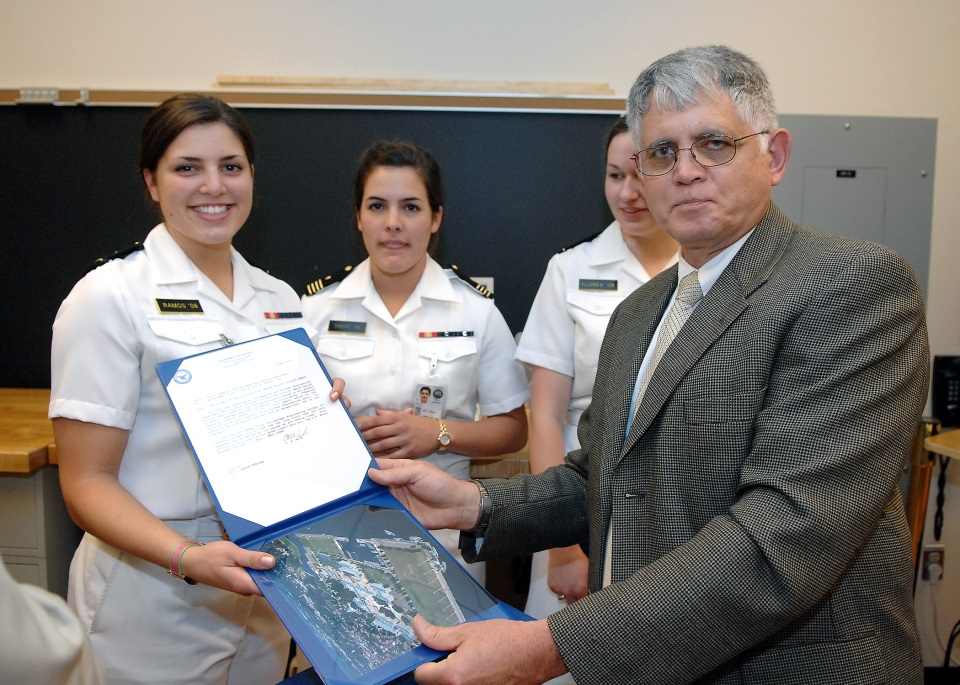
\includegraphics{figures/f6.png}
\end{center}
\caption{Presentation of the 2007 Marsh Award, which is given each year to the best 1/C Systems Engineering project in memory of ENS David R.  Marsh, USNA Class of 1987, in honor of his enthusiasm for his 1/C project, a voice activated robot.}
\label{f6}
\end{figure}

When composing your figures in Inkscape or Adobe Illustrator, use 8 point Arial or Times New Roman for axis label or titles. Use words rather than symbols or abbreviations to avoid confusing the reader. As an example, write the quantity ``Magnetization'', or ``Magnetization, $M$'', not just ``$M$''. If including units in the label, present them within parentheses. Do not label axes only with units. In the example, write ``Magnetization (\si{\ampere\per\meter})'' not just ``\si{\ampere\per\meter}''. Scale the figure appropriately for one or two columns so that they are readable, with thick enough lines and markers, etc. 

With \lstinline{.svg} files, it is possible to include \LaTeX\ and to have it automatically match the font and size with the body of the text when using \lstinline{includesvg}. 

\subsection{References}
Use \lstinline{bibtex}, it's much easier than using the thing built into Word. If you enter things correctly, it will handle the formatting for you. It will also automatically and correctly number the citations. The file \lstinline{example.bib} gives examples of how to code the bibliographic entries. 

To cite them, within the body of your text use the \lstinline|\cite{refname}| command. \LaTeX\ will automatically sort, number, etc. IEEE formats use a reference number within brackets, e.g. \cite{young1964synthetic}. The format of bibliography references can be changed using the \lstinline|\bibliographystyle| command. You may wish to do so if biology-style (Author, 2018) parenthetical references are more appropriate for your subject, for example. 








\end{document}


